\documentclass[11pt,a4paper]{article}

\usepackage[utf8]{inputenc}
\usepackage[T1]{fontenc}
\usepackage[french]{babel}
\usepackage{lmodern}
\usepackage[margin=5em]{geometry}
\usepackage{graphicx}
\usepackage{booktabs}
\usepackage{subcaption}
\usepackage{float}
\usepackage{hyperref}
\hypersetup{hidelinks}
\usepackage{titlesec}

\setlength{\parindent}{0em}
\setlength{\parskip}{1em}
\setlength{\baselineskip}{0em}
\setlength{\columnsep}{0.5em}
\setlength{\tabcolsep}{0.25em}
\titlespacing*{\section} {0pt}{0.1em}{0em}
\titlespacing*{\subsection} {0pt}{0.1em}{0em}

\title{HAI930I - Systèmes multi-agents\\Tournoi d'Axelrod : un LLM auto-adaptatif (MAPE-K)\\face à des stratégies déterministes}
\author{Dejean Robin, Hafdane Léo, Texier-Grailhes Killian}
\date{Novembre 2026}

\begin{document}
\maketitle

\pagenumbering{gobble}
\newpage
\pagenumbering{arabic}

\section{Introduction}

Le projet reproduit le tournoi d'Axelrod sur le dilemme du prisonnier itéré
(gains : 3/3 si les deux coopèrent, 1/1 si les deux trahissent, 5/0 pour celui
qui trahit un coopérateur). Un joueur piloté par un LLM y affronte neuf
stratégies déterministes classiques. À chaque round, le LLM joue selon une
\emph{stratégie de prompt} (Generous, Pragmatic, Merciless ou Peacemaker). Tous
les \texttt{mapek\_every} rounds, une boucle MAPE-K (Monitor, Analyze, Plan,
Execute, Knowledge) peut changer cette stratégie.

La question posée par le sujet est la suivante : \textbf{un LLM auto-adaptatif
  peut-il remonter au score (« comeback ») quand il détecte qu'il joue mal ?}

% ─────────────────────────────────────────────────────────────────────────
\section{Paramètres testés}

Nous avons étudiés les résultats de \textbf{786 matchs} différents en faisant varier les 9 paramètres \ref{tab:parametres}. Nous avons laissé fixe le paramètre \texttt{seuil POOR} à 1.5 point par round qui représente le seuil à partir duquel on considère que le joueur LLM a mal joué. On définit une cellule comme étant un ensemble de paramètres, une configuration.

\subsection{Variables étudiées}

\begin{table}[H]
  \centering
  \begin{tabular}{llp{8.2cm}}
    \toprule
    Paramètre                    & Valeurs testées & Rôle                                                                                                                        \\
    \midrule
    \texttt{adaptive}            & oui / non       & boucle MAPE-K active, ou stratégie de départ conservée tout le match (référence \emph{figée})                               \\
    \texttt{mapek\_every}        & 1, 5, 10        & la boucle tourne tous les $N$ rounds                                                                                        \\
    \texttt{turns}               & 10, 20          & nombre de rounds par match                                                                                                  \\
    \texttt{window}              & 1, 5, 10, 20    & fenêtre glissante de l'étape Monitor (en rounds)                                                                            \\
    \texttt{temperature}         & 0,1, 0,2, 0,9   & température d'échantillonnage du LLM                                                                                        \\
    \texttt{repetitions}         & 1, 5            & nombre de matchs par combinaison                                                                                            \\
    \texttt{stratégie de départ} & 4               & Generous, Pragmatic, Merciless, Peacemaker                                                                                  \\
    \texttt{MAPE-K window}       & 5,10,20         & nombre de rounds précédents pris en compte lors de la décision du MAPE-K                                                    \\
    \texttt{adversaire}          & 9               & Cooperator, Defector, Tit For Tat, Tit For 2 Tats, Suspicious Tit For Tat, Grudger, Alternator, Prober, Win-Stay Lose-Shift \\
    \bottomrule
  \end{tabular}
  \caption{Paramètres que nous avons fait varier.}
  \label{tab:parametres}
\end{table}

\subsection{Métriques}

\begin{itemize}
  \item \textbf{Score moyen par round} du LLM (entre 0 et 5), le critère
        principal. Pour comparer deux modes à armes égales, on fait d'abord la
        moyenne de chaque cellule (adversaire $\times$ stratégie de départ),
        puis on compare les cellules deux à deux.
  \item \textbf{Issue} du match (victoire, nul, défaite) et \textbf{taux de
          coopération}.
  \item \textbf{Comeback} : moyenne des 5 premiers rounds sous 1,5 point par
        round (seuil « POOR »), et moyenne des 5 derniers rounds supérieure d'au
        moins 0,5 point. On utilise une fenêtre de 5 rounds pour toutes les
        conditions, afin qu'elles restent comparables.
  \item \textbf{Changements de stratégie} décidés par la boucle, et
        \textbf{stratégie finale}.
\end{itemize}

% ─────────────────────────────────────────────────────────────────────────
\newpage
\section{Résultats}

% ---------------------------------------------------------------------------
% Figure 1 : score moyen par adversaire et parité des scores (plots 1 et 3)
% ---------------------------------------------------------------------------
\begin{figure}[!h]
  \centering
  \begin{subfigure}[t]{0.48\linewidth}
    \centering
    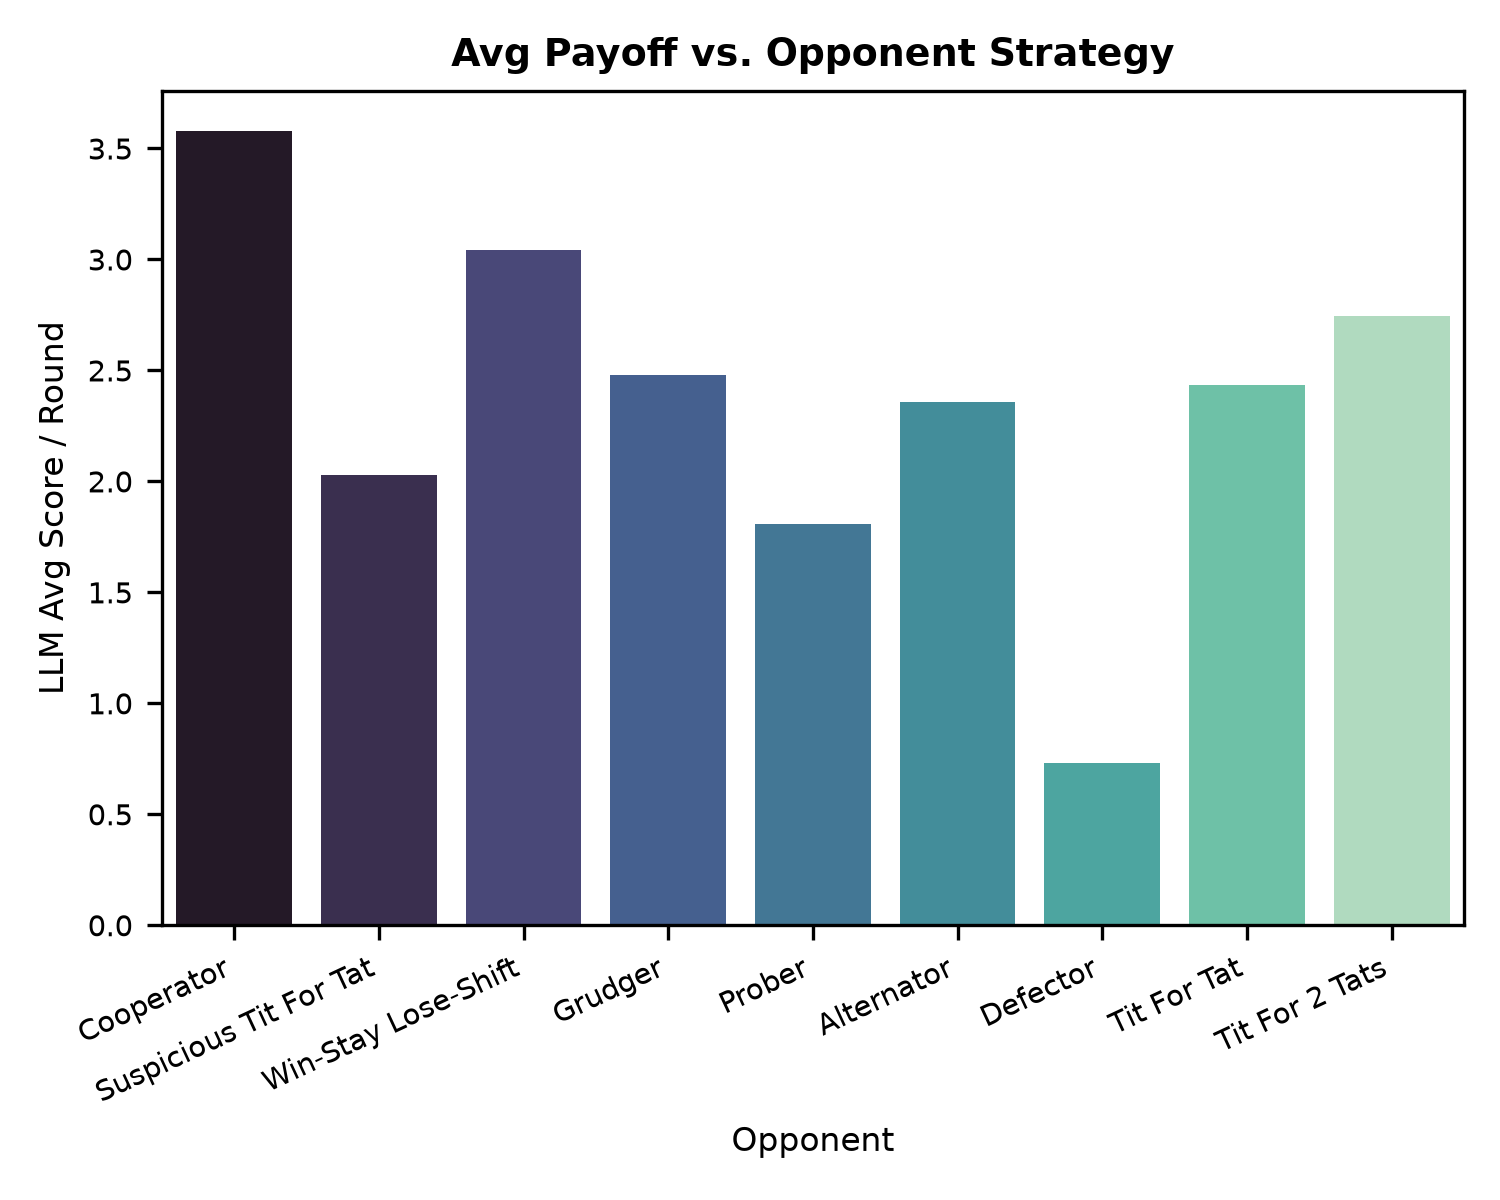
\includegraphics[width=\linewidth]{figures/plot_1_avg_payoff.png}
    \caption{Score moyen par tour du LLM selon la stratégie de
      l'adversaire.}
    \label{fig:avg-payoff}
  \end{subfigure}\hfill
  \begin{subfigure}[t]{0.48\linewidth}
    \centering
    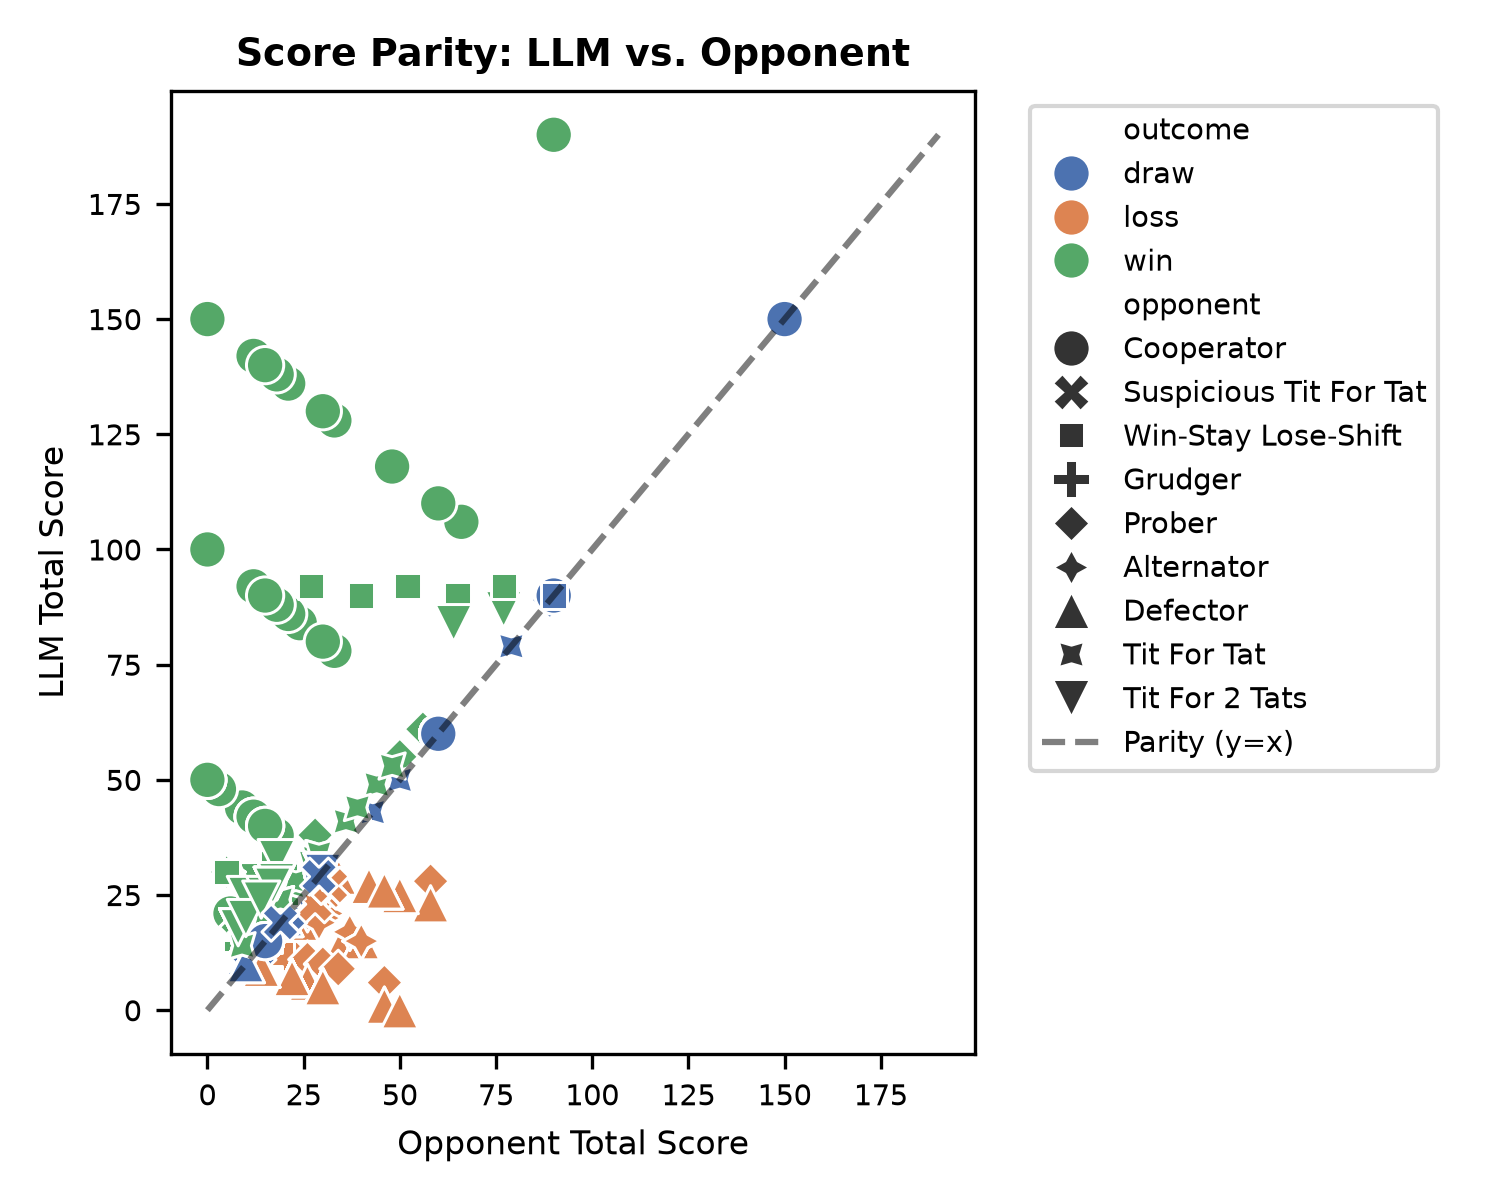
\includegraphics[width=\linewidth]{figures/plot_3_parity.png}
    \caption{Score total du LLM en fonction du score total de l'adversaire
      (couleur : issue du match, symbole : adversaire, pointillés :
      parité).}
    \label{fig:parity}
  \end{subfigure}
  \caption[Scores du LLM selon l'adversaire]{Scores du LLM selon la stratégie
    de l'adversaire. Le meilleur score, et les meilleurs gains, sont obtenus
    contre \texttt{cooperator} ; le pire contre \texttt{defector}. Les autres
    adversaires sont répartis de façon plus uniforme.}
  \label{fig:payoff-parity}
\end{figure}

% ---------------------------------------------------------------------------
% Figure 2 : activité de MAPE-K et gain de l'adaptation (plots 4 et 10)
% ---------------------------------------------------------------------------
\begin{figure}[!h]
  \centering
  \begin{subfigure}[t]{0.48\linewidth}
    \centering
    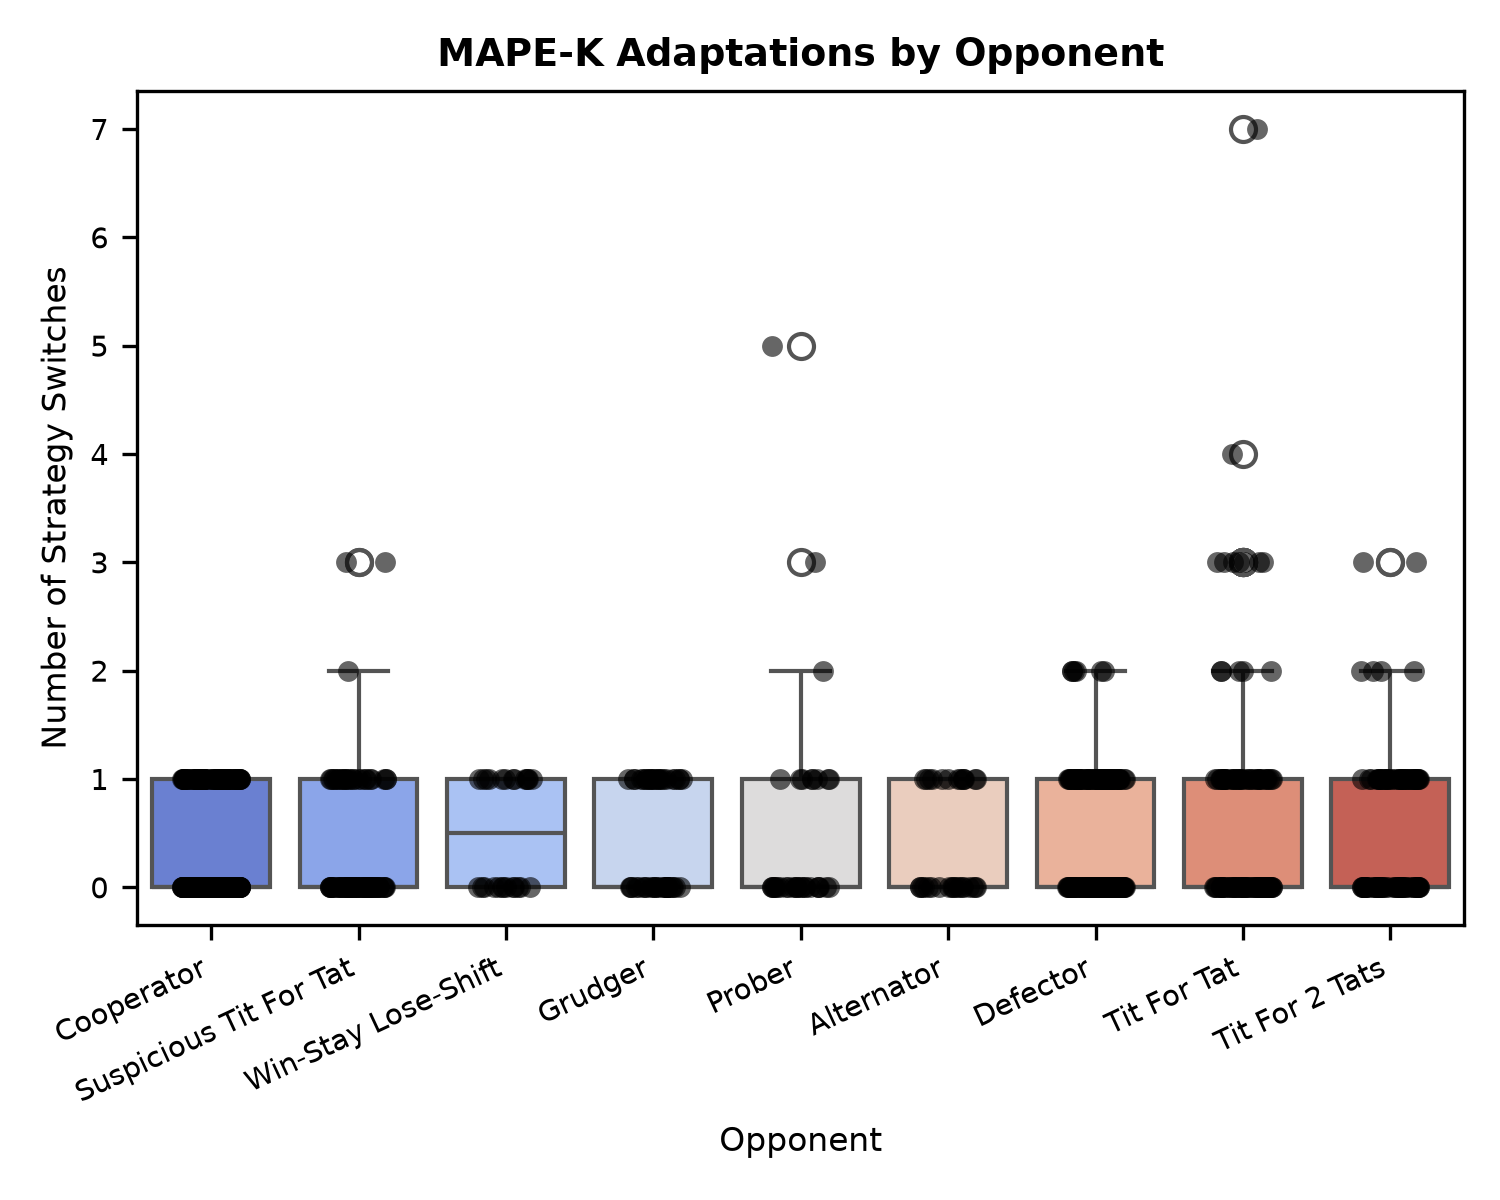
\includegraphics[width=\linewidth]{figures/plot_4_switches.png}
    \caption{Nombre de changements de stratégie de MAPE-K.}
    \label{fig:switches}
  \end{subfigure}\hfill
  \begin{subfigure}[t]{0.48\linewidth}
    \centering
    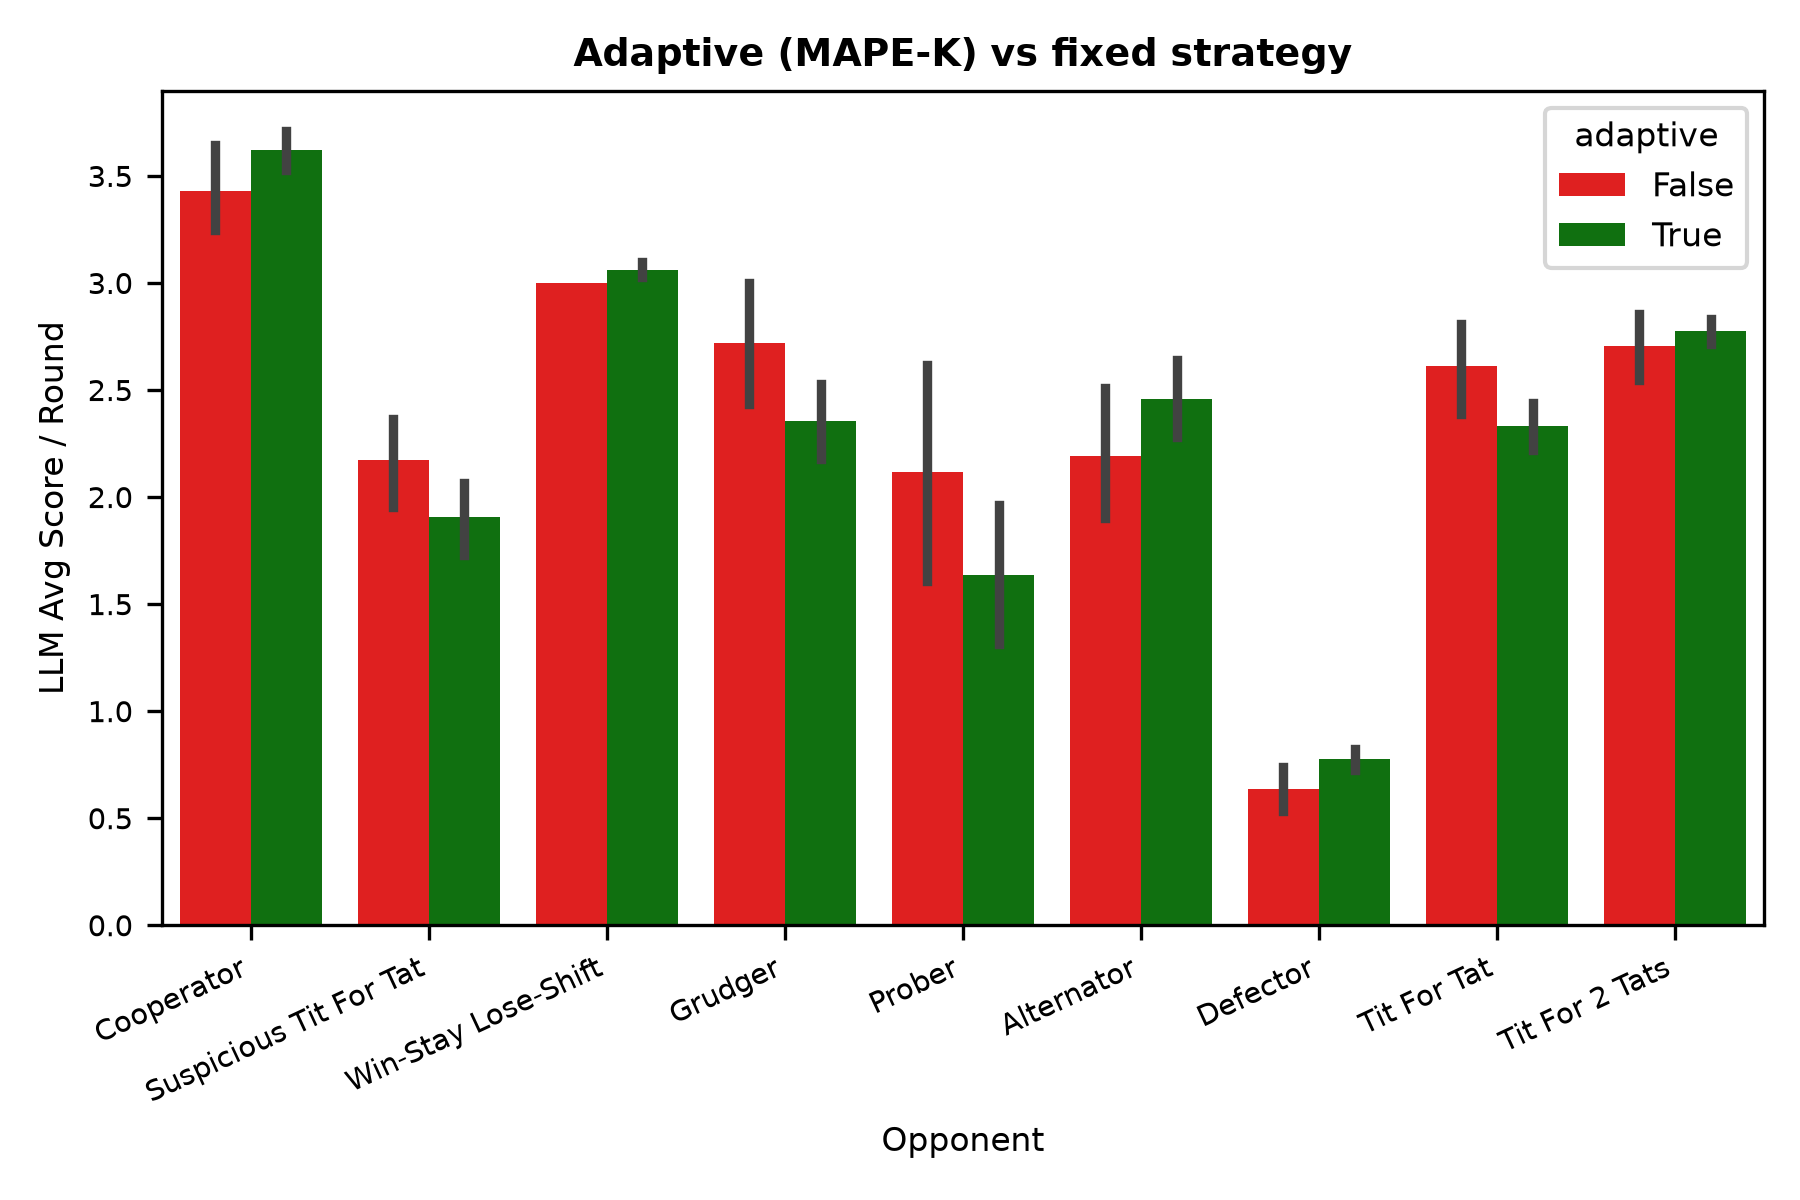
\includegraphics[width=\linewidth]{figures/plot_10_adaptive_vs_fixed.png}
    \caption{Score moyen avec MAPE-K (adaptatif) et sans (stratégie fixe).}
    \label{fig:adaptive-vs-fixed}
  \end{subfigure}
  \caption{Activité de MAPE-K et gain apporté par l'adaptation. On observe une corrélation entre le nombre de changements de stratégie effectués par MAPE-K et l'écart de score avec la version non adaptative. Les adversaires dont la stratégie dépend des actions du LLM, comme \texttt{titfortat}, entraînent davantage de changements de stratégie que les adversaires aux comportements fixes et prévisibles, comme \texttt{cooperator} ou \texttt{defector}. Contre ces stratégies réactives, MAPE-K change fréquemment de stratégie, sans que ces adaptations se traduisent nécessairement par une amélioration du score. À l'inverse, contre les stratégies plus simples, les changements sont moins fréquents et l'adaptation apporte souvent un gain. Nous faisons l'hypothèse que la fenêtre d'observation (window) utilisée par MAPE-K est trop courte pour analyser suffisamment les comportements des adversaires réactifs et identifier des adaptations pertinentes. Cette limite pourrait expliquer pourquoi les changements de stratégie réduisent parfois l'utilité de MAPE-K face à ces adversaires plus complexes.}
  \label{fig:mapek-activity}
\end{figure}

% ---------------------------------------------------------------------------
% Figure 3 : stratégies sur lesquelles MAPE-K converge (plots 5, 7 et 8)
% ---------------------------------------------------------------------------
\newpage
\begin{figure}[!h]
  \centering
  \begin{subfigure}[t]{0.48\linewidth}
    \centering
    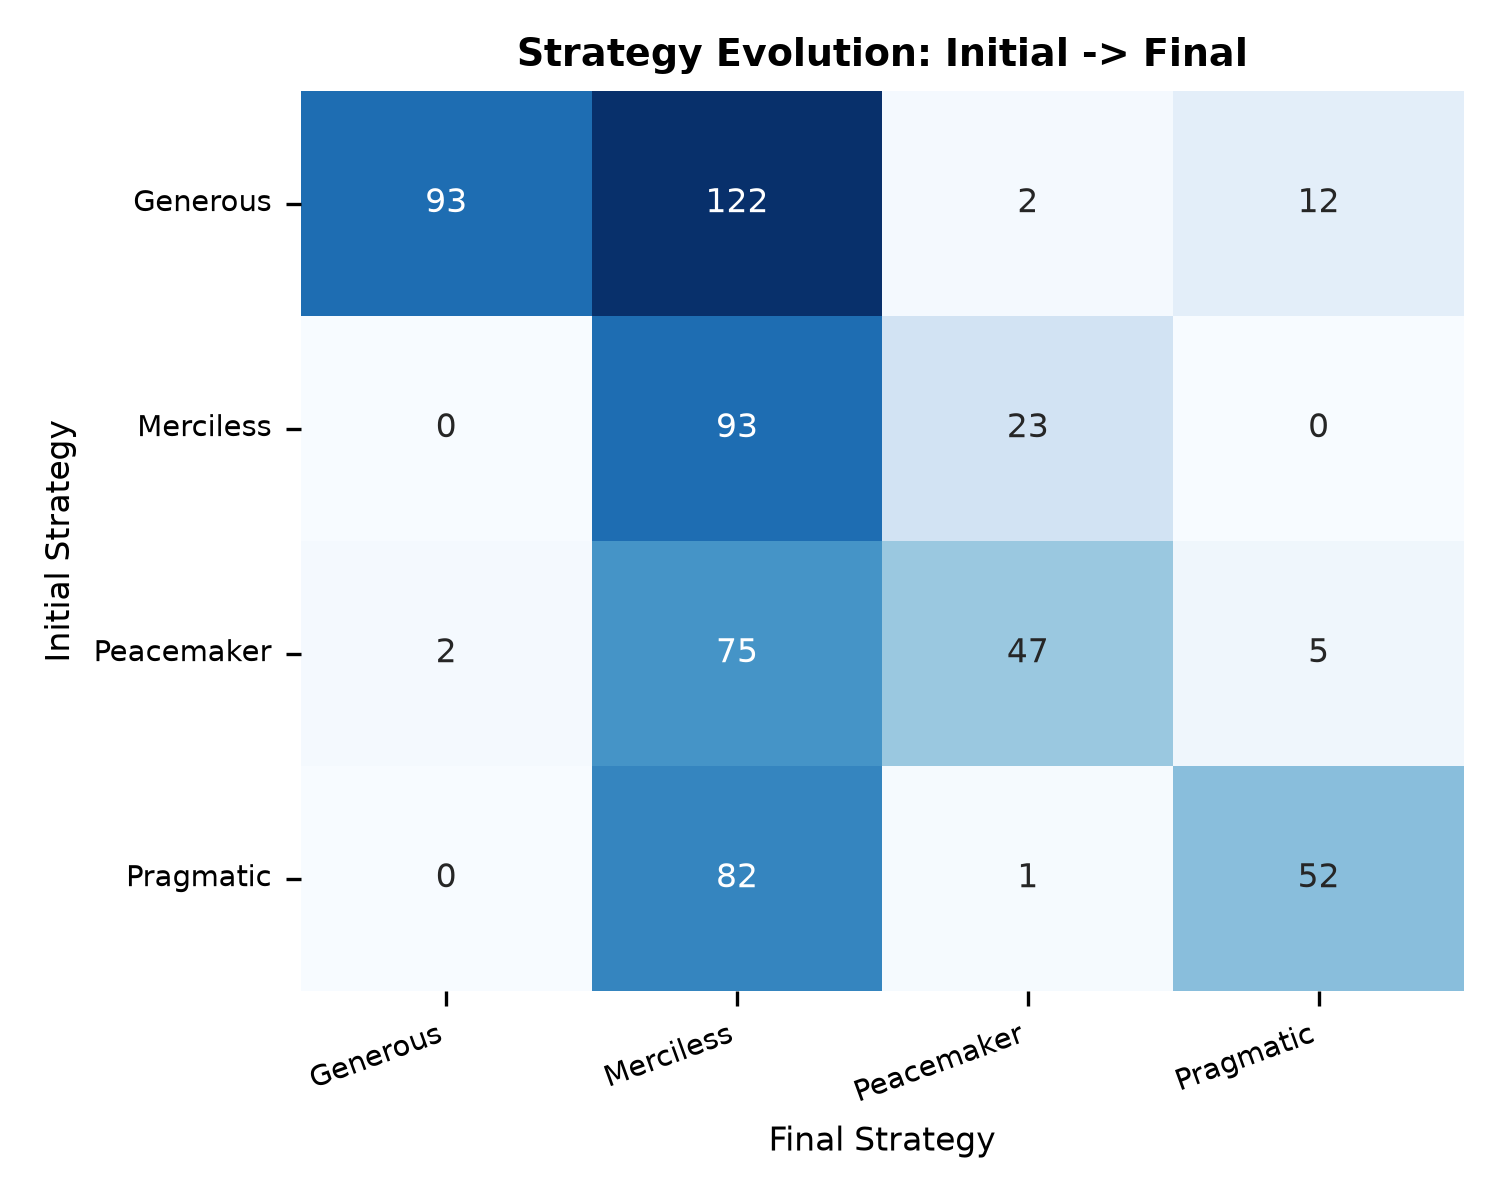
\includegraphics[width=\linewidth]{figures/plot_5_evolution.png}
    \caption{Stratégie initiale $\rightarrow$ stratégie finale (nombre de
      parties).}
    \label{fig:evolution}
  \end{subfigure}\hfill
  \begin{subfigure}[t]{0.48\linewidth}
    \centering
    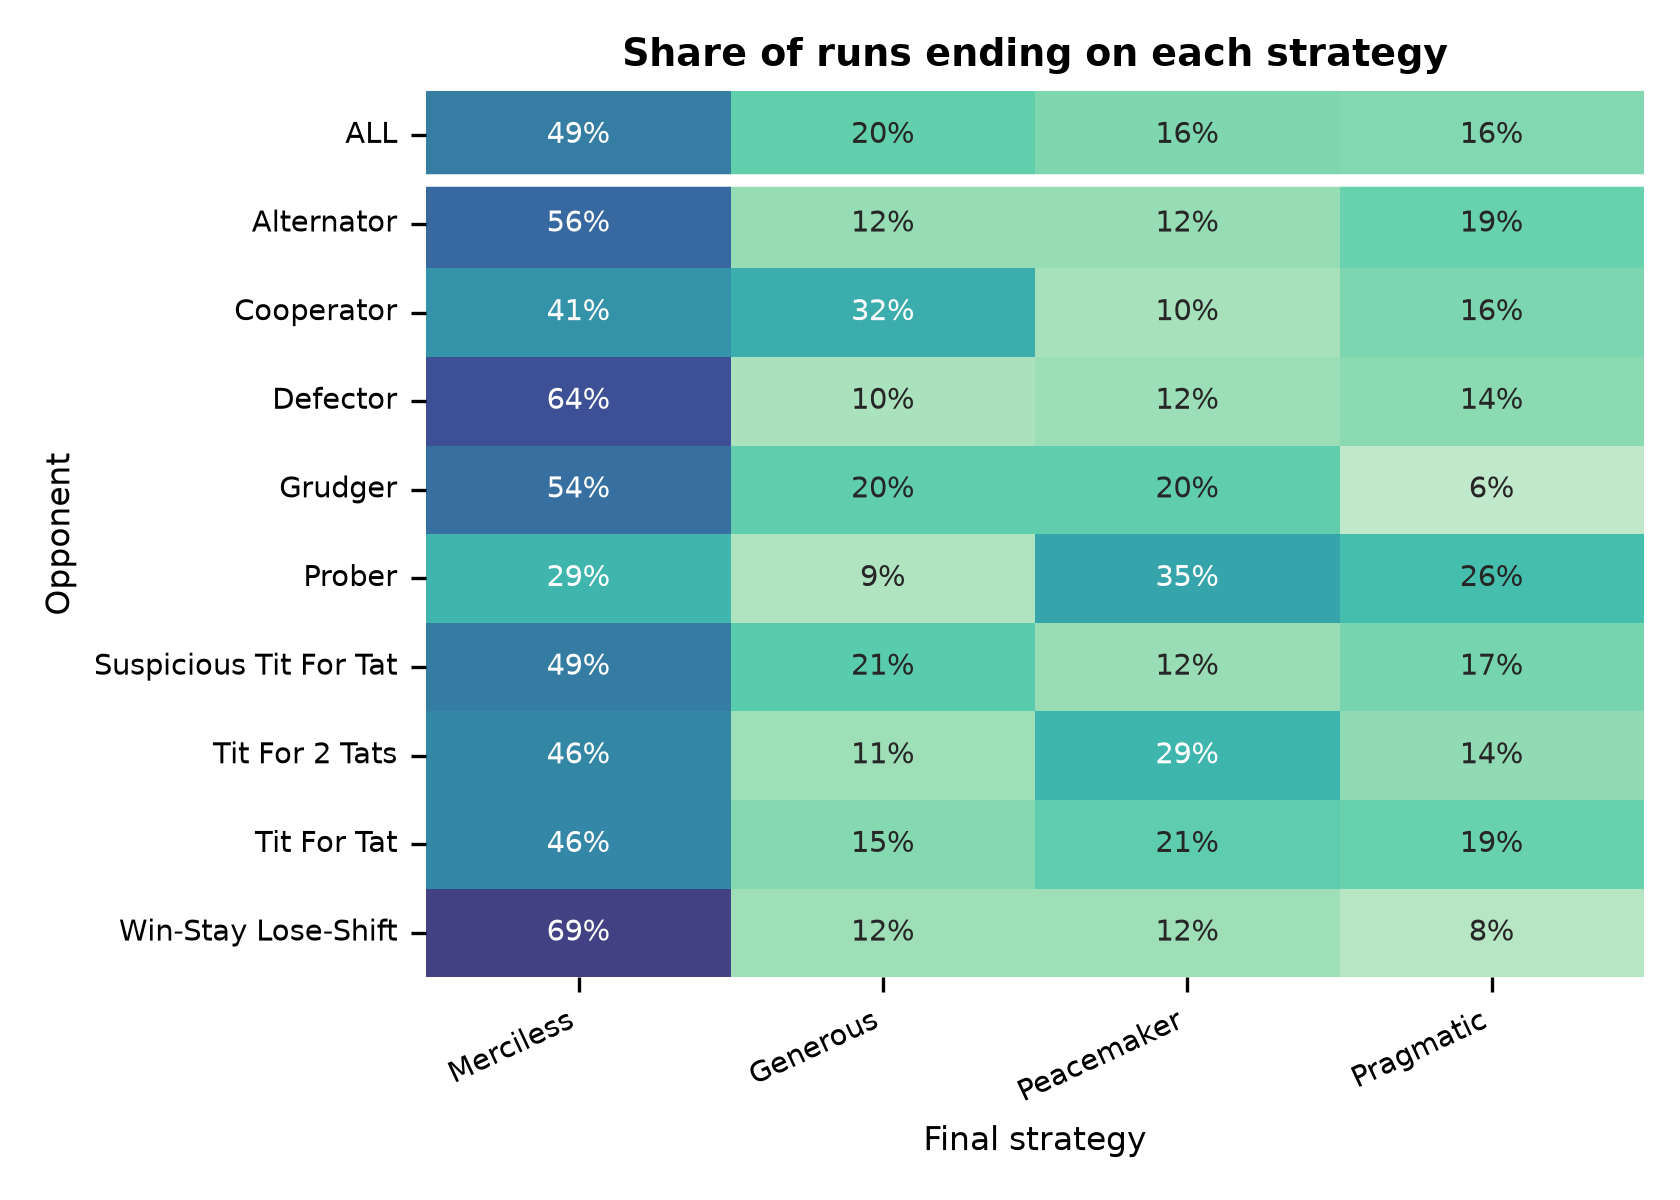
\includegraphics[width=\linewidth]{figures/plot_7_final_strategy_share.png}
    \caption{Part des parties terminées sur chaque stratégie, par adversaire.}
    \label{fig:final-share}
  \end{subfigure}

  \medskip
  \begin{subfigure}[t]{0.85\linewidth}
    \centering
    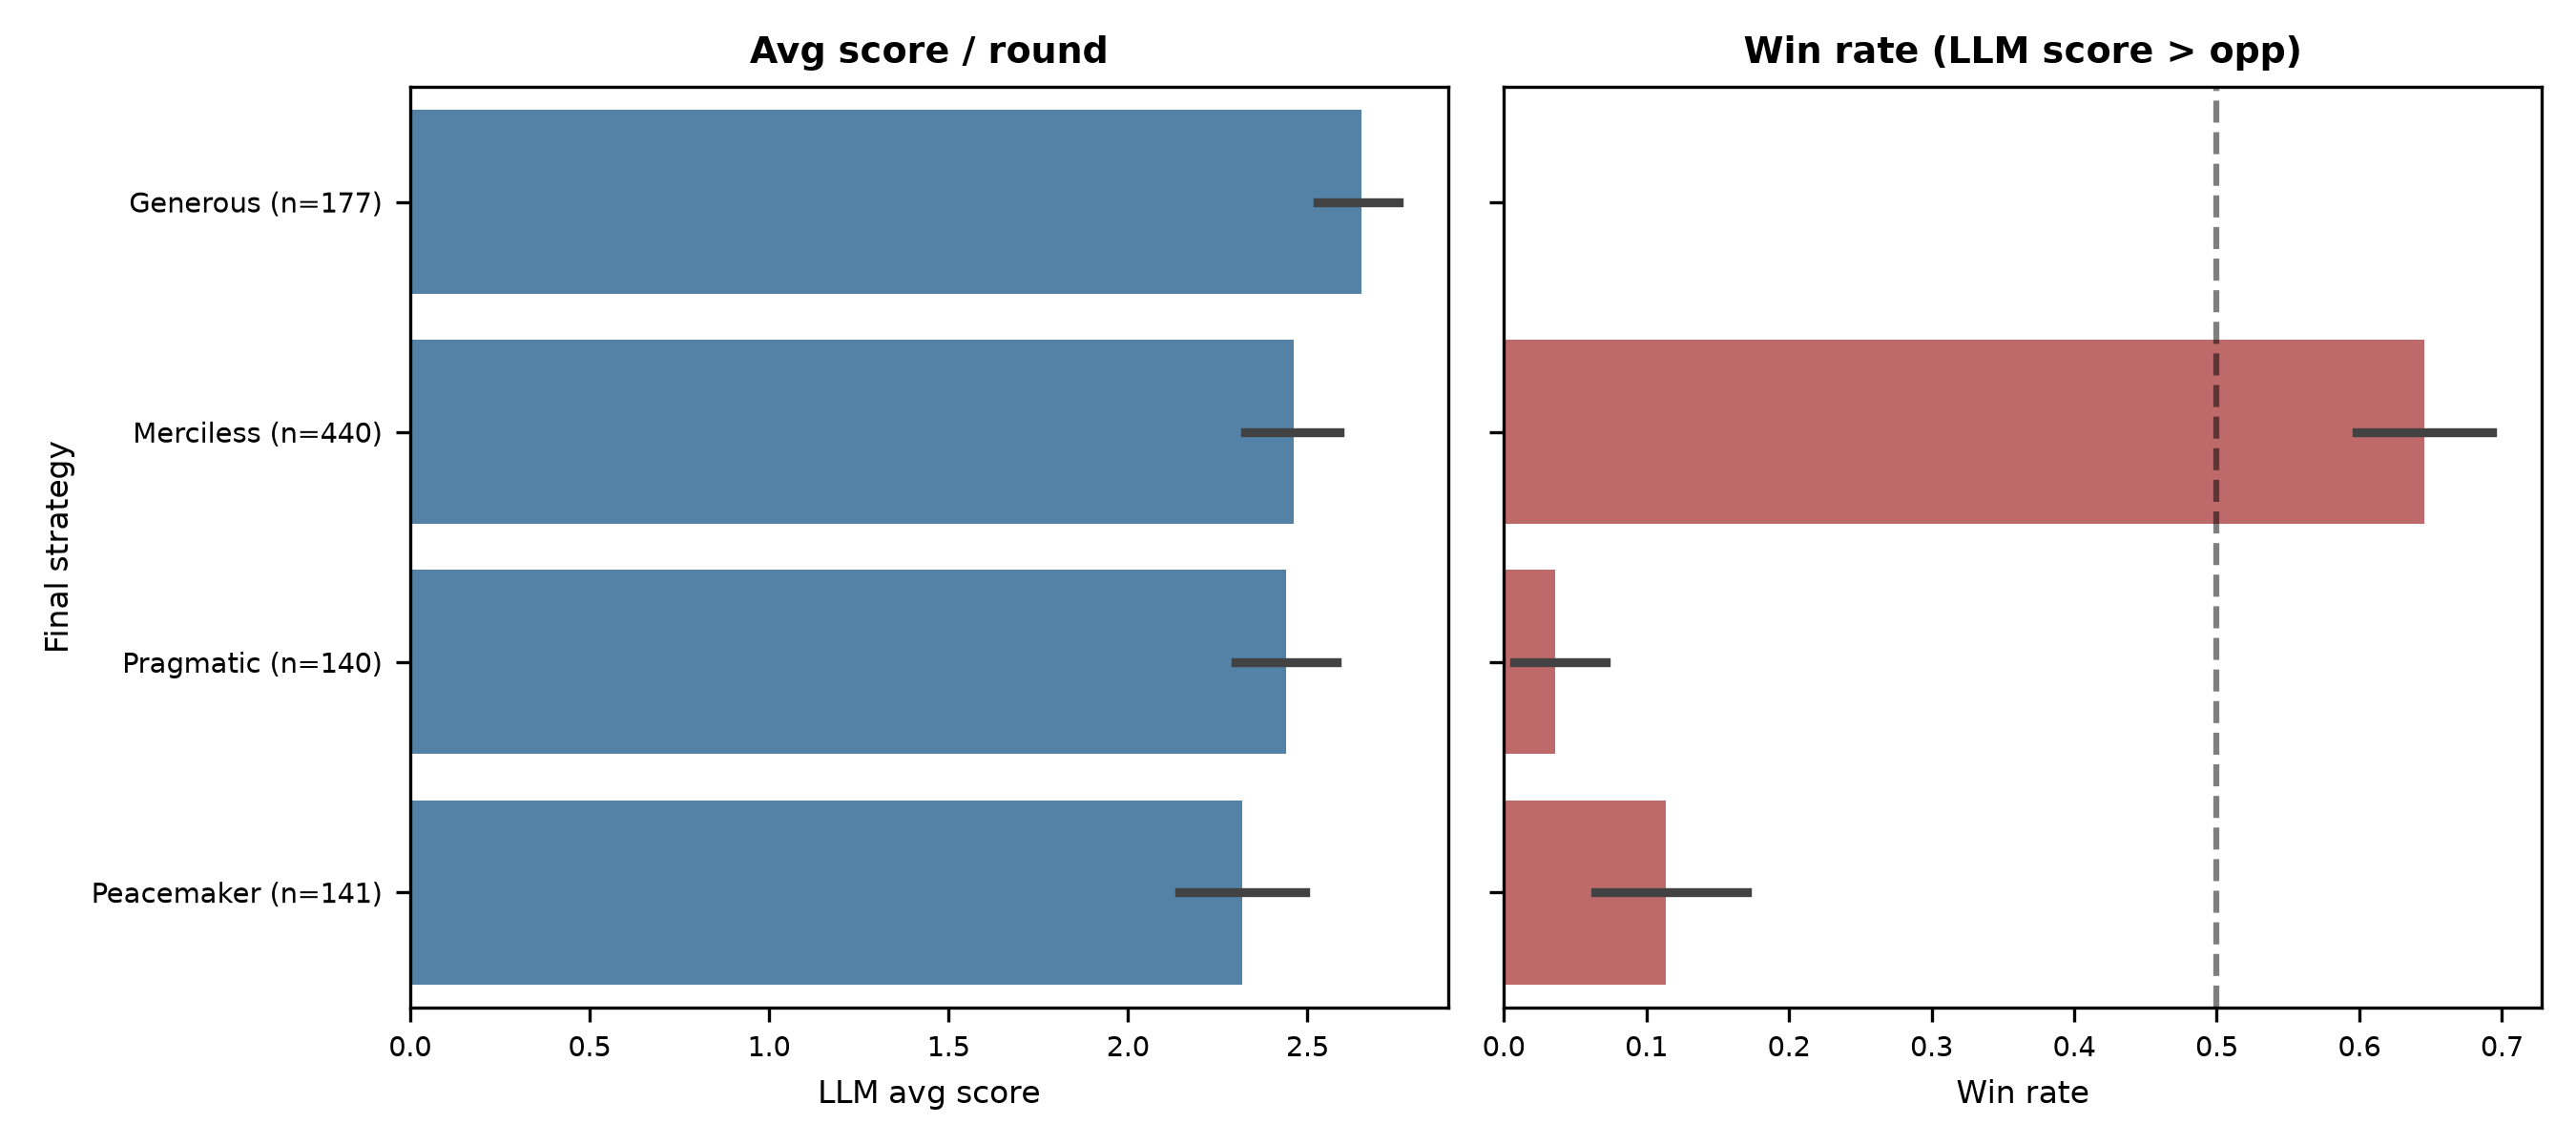
\includegraphics[width=\linewidth]{figures/plot_8_strategy_ranking.png}
    \caption{Classement des stratégies finales : score moyen par tour (à
      gauche) et taux de victoire (à droite).}
    \label{fig:strategy-ranking}
  \end{subfigure}
  \caption[Stratégies sur lesquelles MAPE-K converge]{Stratégies sur
    lesquelles MAPE-K converge. Quels que soient la stratégie de départ et
    l'adversaire, MAPE-K retombe majoritairement sur \texttt{merciless}, la
    stratégie qui a le meilleur taux de victoire. Ce n'est pourtant pas celle
    qui a le meilleur score moyen : contre des adversaires coopératifs,
    \texttt{generous} fait fortement augmenter sa moyenne, mais elle ne gagne
    jamais (défaite ou égalité).}
  \label{fig:strategy-convergence}
\end{figure}

% ---------------------------------------------------------------------------
% Figure 4 : interactions entre paramètres (plot 12)
% ---------------------------------------------------------------------------

\newpage

\begin{figure}[!h]
  \centering
  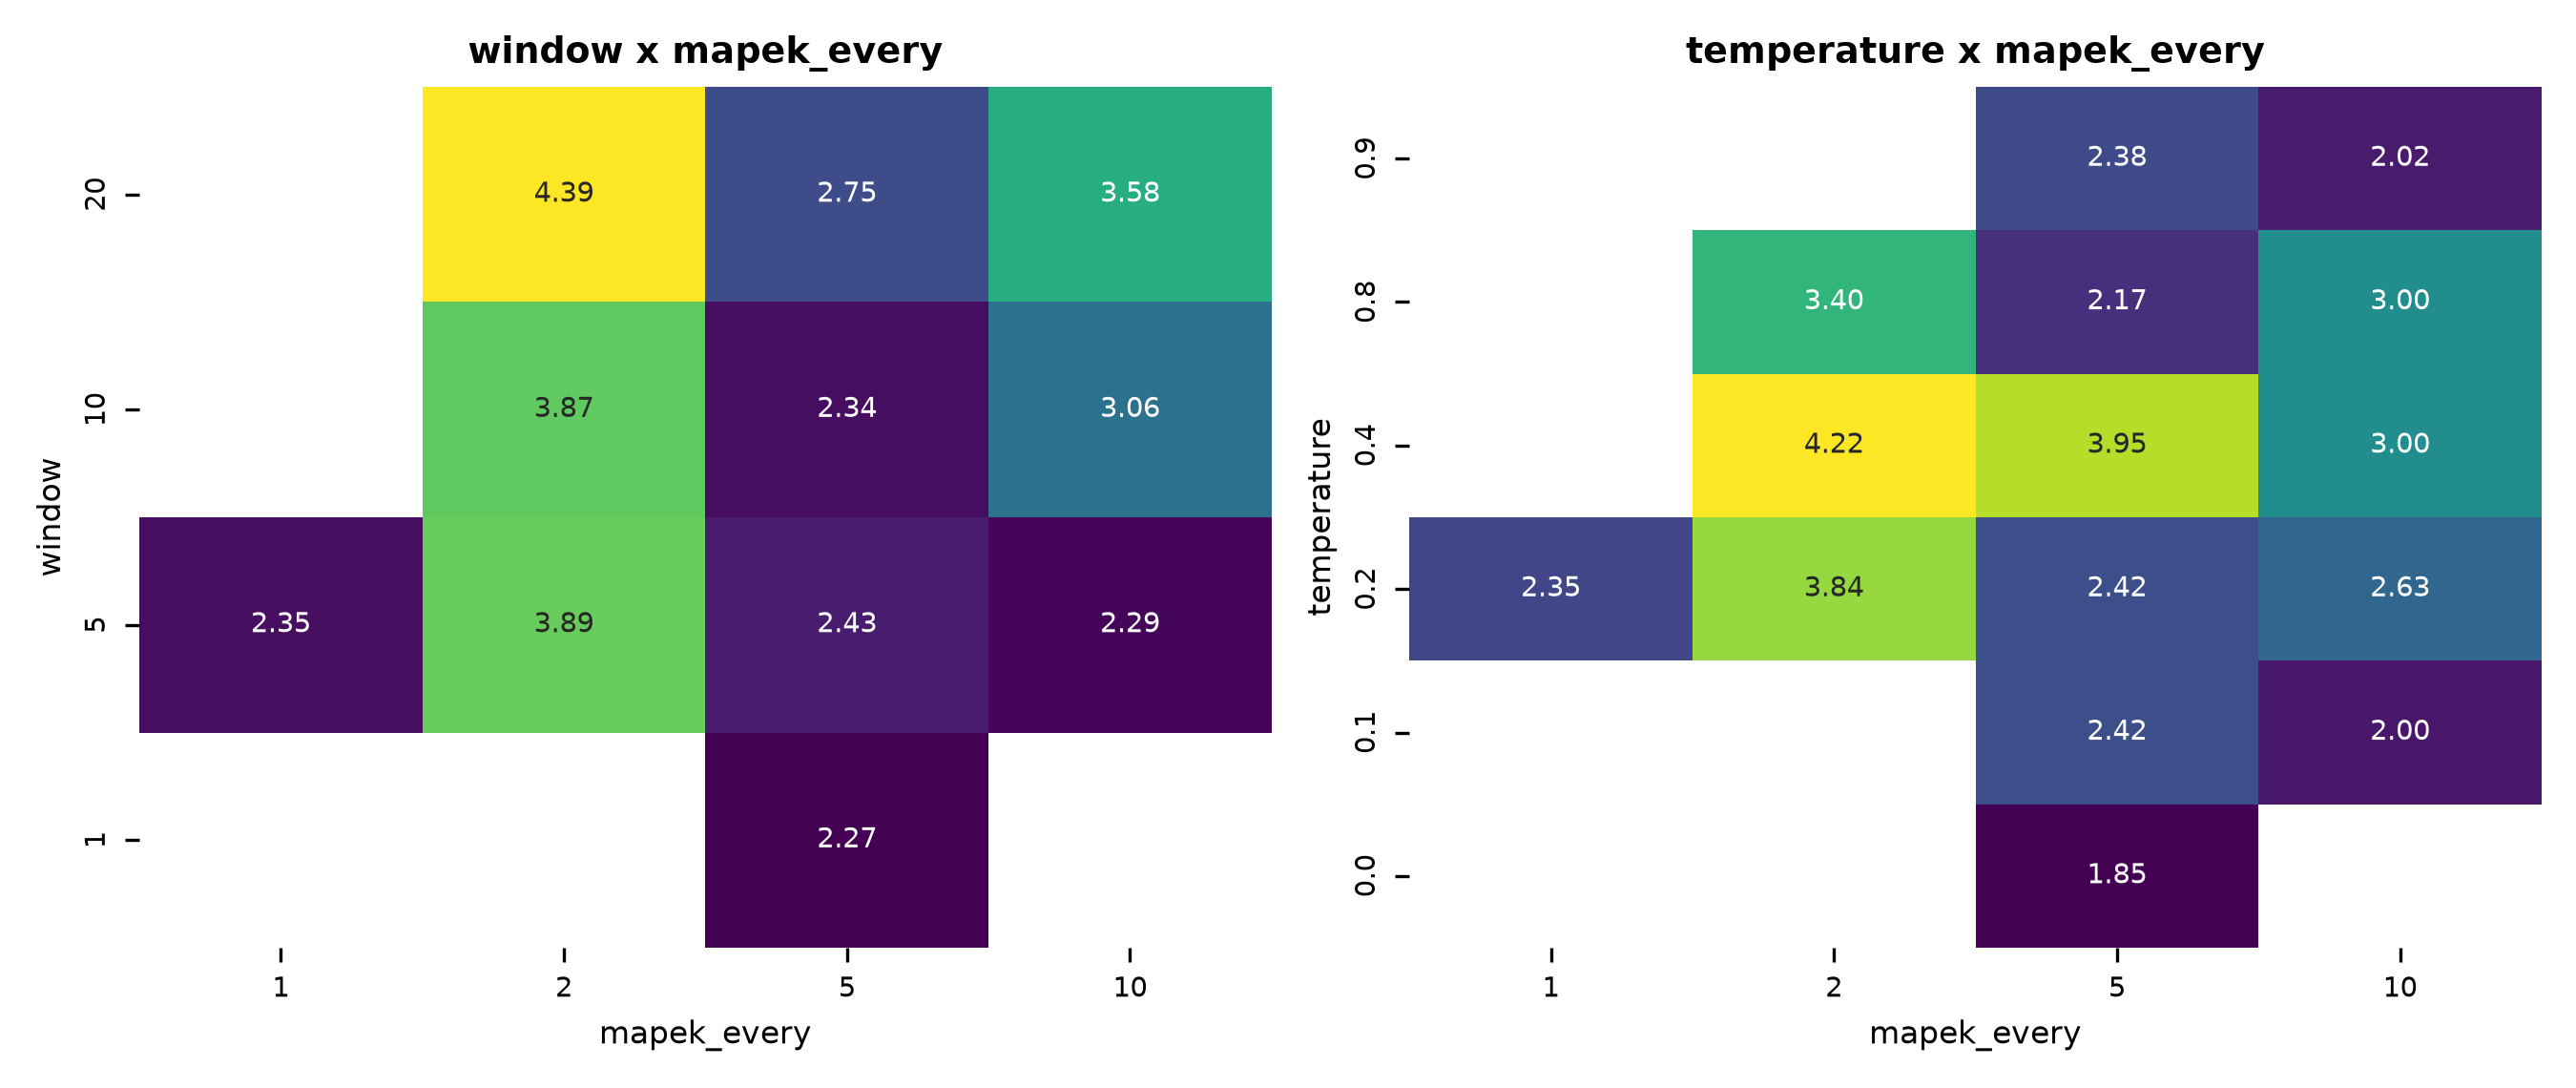
\includegraphics[width=\linewidth]{figures/plot_12_param_interactions.png}
  \caption[Influence des paramètres de MAPE-K et du LLM]{Score moyen par tour
    selon les paires de paramètres (\texttt{mapek\_every}, \texttt{window},
    \texttt{poor\_threshold}, \texttt{temperature}). Les meilleurs résultats
    sont obtenus pour \texttt{mapek\_every}\,$=2$ (il vaut probablement mieux
    déclencher MAPE-K plus souvent), pour une \texttt{window} plus grande, et
    pour une température du LLM de $0{,}4$. Attention : le nombre de parties
    par case est faible, ces tendances sont donc à confirmer avec davantage de
    données.}
  \label{fig:param-interactions}
\end{figure}

% ---------------------------------------------------------------------------
% Figure 5 : comebacks percentages (plot 16)
% ---------------------------------------------------------------------------
\begin{figure}[!h]
  \centering
  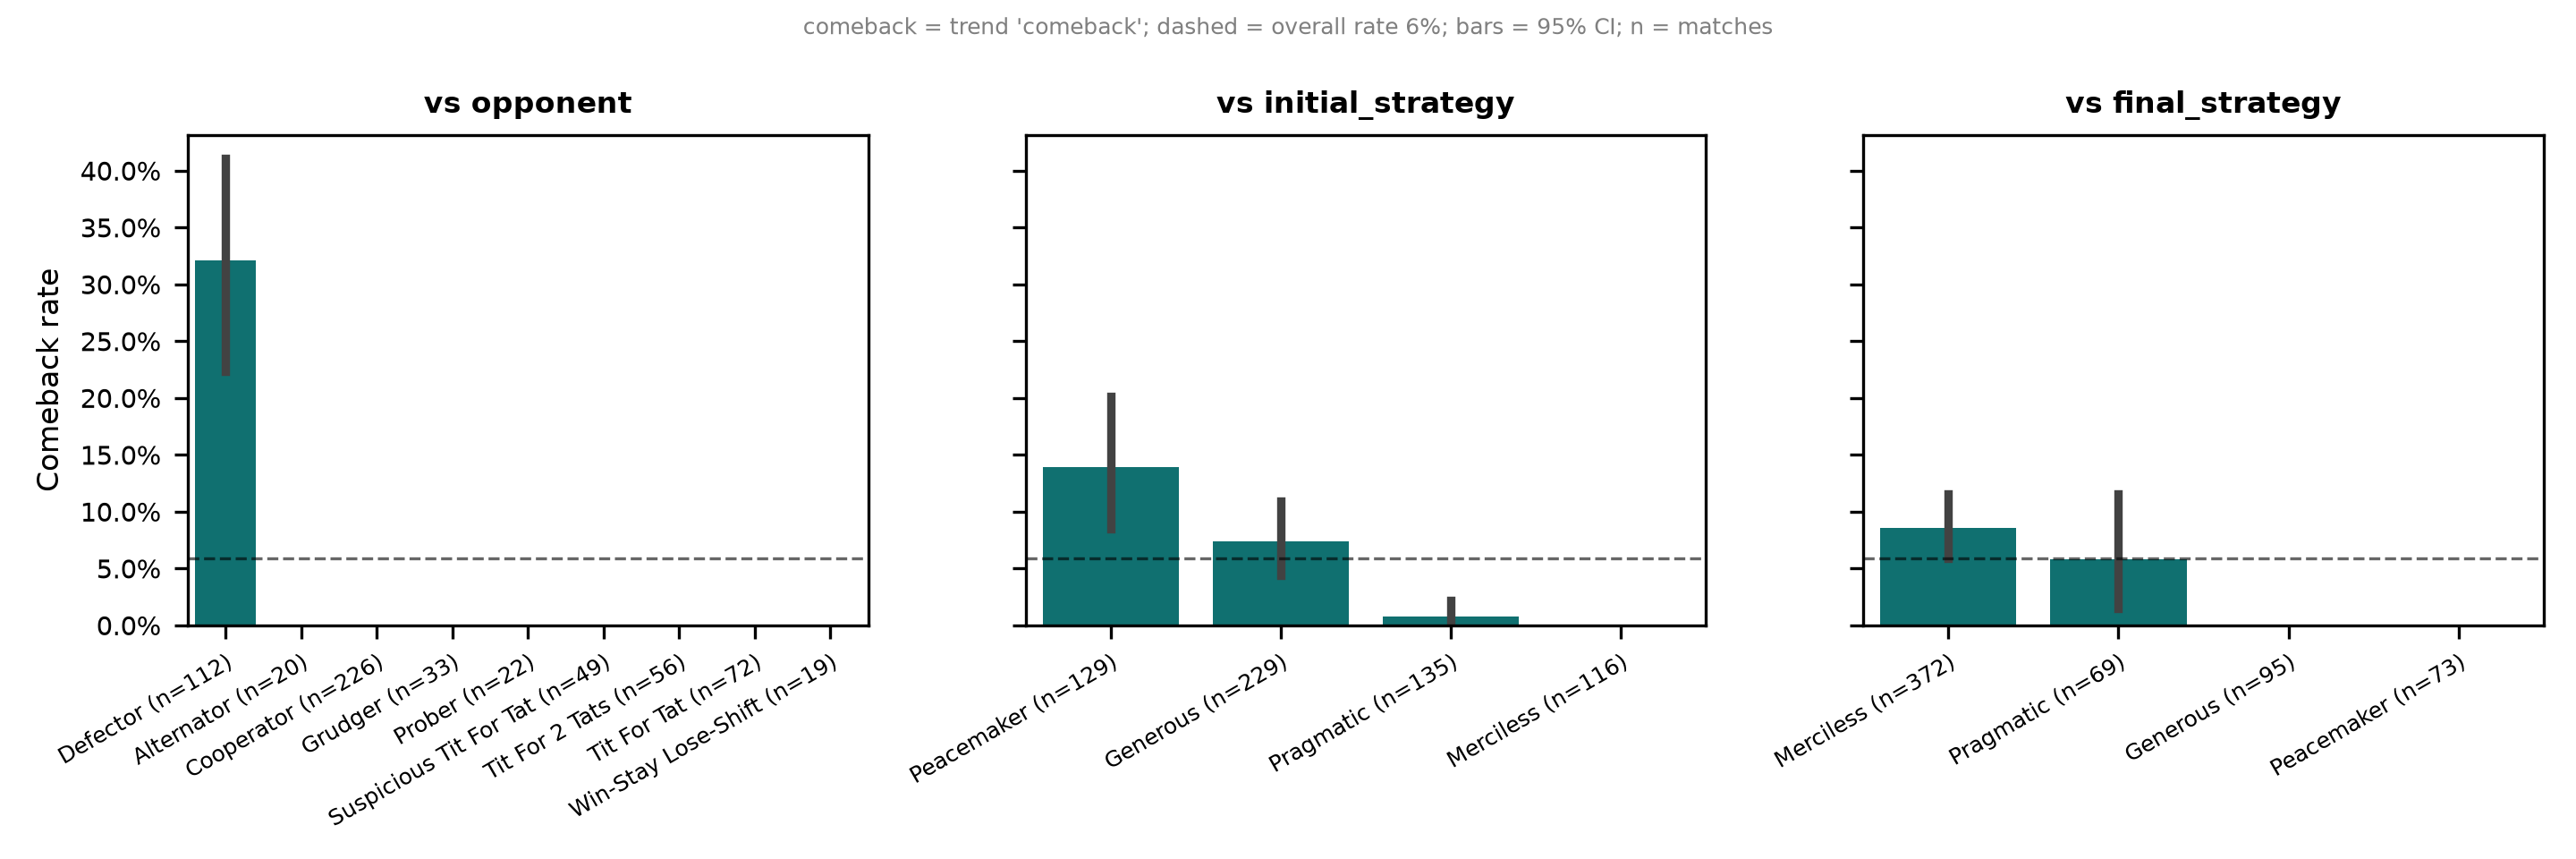
\includegraphics[width=\linewidth]{figures/plot_16_comeback_drivers.png}
  \caption{Le comeback est presque uniquement possible contre \texttt{Defector} car c'est le seul qui mets dans un premier temps en difficulté sans s'adapter par la suite (reste prévisible). On voit bien que les stratégies nulles (\texttt{Peacemaker} et \texttt{Generous}) comebackent en basculant vers les stratégies fortes (\texttt{Pragmatic} et \texttt{Merciless})}
  \label{fig:comebacks}
\end{figure}

% ─────────────────────────────────────────────────────────────────────────
\section{Conclusion}

\subsection{Réponse à la question}

\textbf{Oui, un LLM auto-adaptatif peut remonter au score quand il détecte
  qu'il joue mal.} Quand le LLM se fait exploiter (par Defector, dans nos
expériences), la boucle MAPE-K le détecte et change de stratégie : 46\,\% des
matchs mal commencés se terminent en comeback, contre 5\,\% sans adaptation. Le
LLM atteint alors le meilleur score possible contre cet adversaire. Avec une
boucle à chaque round, il réagit encore plus tôt et évite une bonne partie de
la perte de points (0,91 point par round contre Defector, au lieu de 0,41 en
figé).

\textbf{Mais ce comeback ne rend pas le LLM meilleur en général.} Sur
l'ensemble des adversaires, la boucle ne change pas le score moyen (écart
de 0,00 point par round). La raison est un \textbf{biais marqué de l'étape Plan
  vers Merciless} (68\,\% des matchs adaptatifs finissent dans cette stratégie) :
le LLM trahit aussi quand tout va bien, ce qui casse la coopération avec les
stratégies qui punissent la trahison (Grudger, Tit For Tat, Suspicious Tit For
Tat). Il gagne plus de matchs (47\,\% contre 17\,\%) mais ne marque pas plus de
points. Dans l'esprit du tournoi d'Axelrod, où seul compte le total de points,
l'adaptation n'apporte donc pas d'avantage.

\textbf{Stratégies optimales observées} : Merciless contre les adversaires
inconditionnels (Cooperator, Defector, Alternator) ; une stratégie coopérative
et réciproque (Pragmatic, Peacemaker ou Generous) contre les stratégies qui
punissent la trahison. Une boucle idéale devrait donc identifier la famille de
l'adversaire et \emph{ne pas} quitter une coopération mutuelle qui fonctionne.

\subsection{Limites et pistes}

\begin{itemize}
  \item \textbf{Matchs courts.} Avec 10 rounds et une boucle tous les 5 rounds,
        le LLM ne peut changer de stratégie qu'une fois. Les matchs de 20 rounds
        n'ont été joués que contre 3 adversaires et sans référence figée.
  \item \textbf{Modèles.} Ils ne se comportent pas pareil dans l'étape Plan, et
        le modèle utilisé est lié à certaines conditions. Une même série
        d'expériences devrait être jouée avec un seul modèle.
  \item \textbf{Échantillons.} Avec 1 répétition, chaque cellule ne contient
        que 1 à 3 matchs : les écarts de quelques centièmes ne sont pas
        significatifs. Seules les tendances retrouvées dans plusieurs conditions
        (par famille d'adversaires, comeback contre Defector, biais vers
        Merciless) sont solides.
  \item \textbf{Tournoi.} Aucun tournoi n'a été joué avec une boucle active.
\end{itemize}

\paragraph{Pistes.} Rendre l'étape Plan plus prudente (ne pas quitter une
stratégie qui donne un résultat « GOOD », ou garder la coopération mutuelle
comme objectif). Allonger les matchs et ajouter une référence figée de même
longueur. Rejouer les tournois avec une boucle active (par exemple tous les
5 rounds sur 30 rounds). Intégrer les résultats de Léo, qui ne figurent pas
encore dans ces données.

\end{document}
